\chapter{Mathematischer Teil II – Die Bedeutung von $\alpha^*$}
\label{chap:mathematischer_rahmen_II}

\section{Empirischer Bezug – Wechselspannung als Energie‐Zeit‐Symmetrie}

Im vorangegangenen Kapitel wurde gezeigt, dass sich durch numerische Rasterung
über acht Raumrichtungen hinweg ein konstanter Operator identifizieren lässt,
dessen Wert $\alpha^*$ eine außergewöhnliche Skalenkonstanz über atomare,
nukleare und kosmologische Energiesysteme zeigt.
Um die physikalische Bedeutung dieses Operators zu klären,
bietet sich ein empirisch gut zugängliches Energiesystem an,
in dem Energie und Zeit periodisch gekoppelt sind:
das elektrische Wechselspannungsfeld.

\begin{figure}
  \centering
  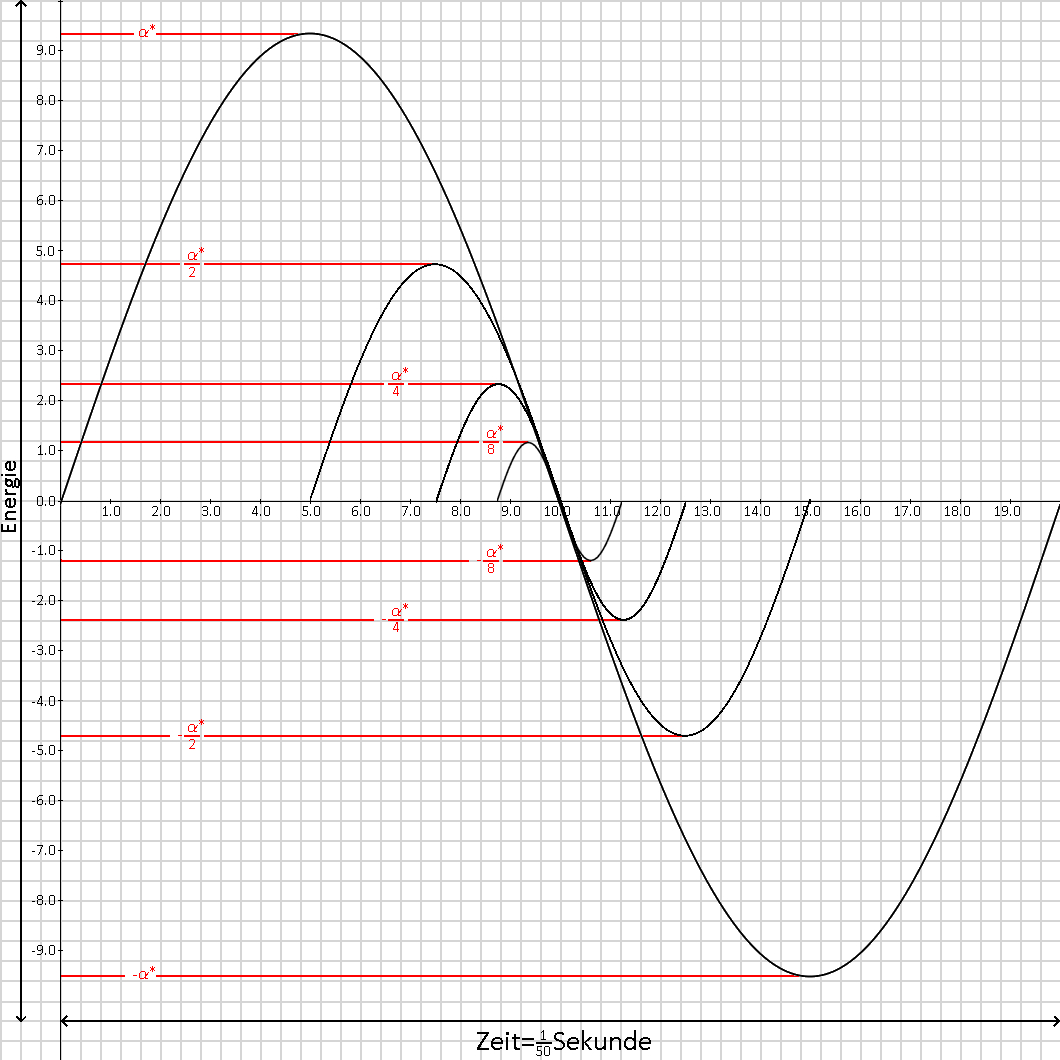
\includegraphics[width=0.85\textwidth]{Grafiken/Wechselspannung.jpg}
  \caption{Das normierte Wechselpannungsfeld enthält $\alpha^*$}
  \label{Diagramm1}
\end{figure}

Eine Wechselspannung beschreibt das zeitlich alternierende Potential
\[
U(t) = U_0 \sin(\omega t).
\]
Die Energie folgt dabei der quadratischen Form
\[
E(t) \propto U^2(t),
\]
wodurch sich eine periodische Energie–Zeit–Symmetrie ergibt.
Wird diese über mehrere Phasen hinweg verschoben,
entsteht eine geordnete, zeitlich und räumlich
symmetrische Energieverteilung.
Damit bildet die Wechselspannung eine natürliche Referenz
für das, was hier als \emph{aperiodische Energie–Zeit–Symmetrie}
der Realität verstanden wird.

Das elektrische Dreiphasensystem (Drehstrom)
stellt die empirische Analogie zum dreidimensionalen Raum dar:
drei zueinander phasenverschobene sinusförmige Potentiale,
deren gemeinsame Überlagerung eine stabile, rotierende
Energiekonfiguration erzeugt.
Dieses Verhalten deutet darauf hin, dass reale Energiesysteme
in drei Dimensionen einer übergeordneten geometrischen Symmetrie folgen,
in der Phasenwinkel und Raumrichtungen unmittelbar gekoppelt sind.

\section{Einführung des Operators $\alpha^*$}

Der empirische Fit über verschiedene Energieskalen
führte auf einen dimensionslosen Operator
\[
\alpha^* = 9{,}43034098\dots
\]
der in allen getesteten Domänen (atomar, nuklear, kosmologisch)
als skalierungsstabiler Eigenwert auftritt.
In energetischer Interpretation beschreibt $\alpha^*$
ein konstantes Verhältnis von Energie zu Zeit.
Formal lässt sich schreiben:
\[
\alpha^* = \frac{E}{T},
\]
wobei $E$ die mittlere Energiedichte
und $T$ der effektive Zeitintervall der Resonanz ist.
Damit wird $\alpha^*$ zur \emph{energetischen Frequenzkonstante}
des Raumes selbst.

\section{Das Dreiphasensystem und der Winkelbezug}

Überträgt man den Befund auf das Dreiphasensystem,
so zeigt sich, dass drei periodische Signale
\[
U_i(t) = U_0 \sin(\omega t + \phi_i),
\qquad
\phi_i = \{0,\,120^\circ,\,240^\circ\}
\]
ein vollständiges symmetrisches Energiesystem bilden.
Dieses System erzeugt eine rotierende Feldstruktur,
die in allen drei Raumrichtungen denselben Energieverlauf besitzt.
Die 120°‐Phasenverschiebung lässt sich dabei
als projektiver Anteil eines übergeordneten Öffnungswinkels interpretieren.
Setzt man $\alpha^*$ in Relation zur vollen Kreisphase $360^\circ$,
so ergibt sich
\[
\frac{\alpha^*}{360^\circ} = 0{,}0261953916\dots
\]
und der daraus abgeleitete Öffnungswinkel
\[
\theta^* = 360^\circ \cdot \frac{\alpha^*}{10} = 20{,}50772472^\circ.
\]
Dieser Winkel beschreibt die aperiodische Abweichung
von einer idealen Periode 10
und bildet somit die geometrische Interpretation
des empirisch gefundenen Operators.

\section{Herleitung der Spiralis‐Funktion mit $\alpha^*$}

Die klassische Sinusfunktion
\[
s(\xi) = \sin(2\pi\,\xi)
\]
beschreibt eine periodische Schwingung in einer Dimension.
Für reale Energiesysteme muss jedoch berücksichtigt werden,
dass Raum und Zeit untrennbar gekoppelt sind
und die Schwingung nicht in einer Ebene,
sondern entlang einer räumlichen Spirale verläuft.
Diese Spiralität führt zur beobachteten Aperiodizität der Realität.

Die \emph{Spiralis‐Funktion} verallgemeinert den Sinus
auf einen aperiodischen, dreidimensionalen Verlauf.
Dazu wird die Phase nicht mehr durch $2\pi$ bestimmt,
sondern durch den empirischen Öffnungswinkel $\alpha^*$.
Für eine Dimension ergibt sich:
\[
\mathcal{S}_1(x) = \sin\!\left(\frac{\alpha^*}{3}\frac{\pi}{180}\,x\right),
\]
für zwei Dimensionen:
\[
\mathcal{S}_2(x,y) = \sin\!\left(\frac{\alpha^*}{2}\frac{\pi}{180}\,(x+y)\right),
\]
und für drei Dimensionen:
\[
\boxed{
\mathcal{S}_3(x,y,z)
= \sin\!\left(\alpha^*\frac{\pi}{180}\,(x+y+z)\right).
}
\]
Die dreidimensionale Spiralis bildet damit
die energetische Grundform des Raumes.
Ihre Aperiodizität erklärt,
warum keine natürlichen Systeme exakt periodisch erscheinen
und warum reale Resonanzen stets einen Spiralcharakter besitzen.

\section{Eigenschaften und Bedeutung der Spiralis‐Geometrie}

Die Spiralis‐Geometrie besitzt mehrere bemerkenswerte Eigenschaften:

\begin{enumerate}
\item \textbf{Aperiodizität:}
Die Funktion wiederholt sich nicht exakt;
sie nähert sich einer Periode nur asymptotisch.
Dies spiegelt das Verhalten realer Umlaufbahnen,
Rotationen und Schwingungen wider.

\item \textbf{Symmetrie:}
In drei Dimensionen ergeben sich acht stabile Richtungen
(Octants), in denen die Spiralis‐Welle
überlagerungsstabil ist.
Dies führt zur beobachteten 8‐fachen Symmetrie
in den numerischen Simulationen.

\item \textbf{Hierarchie:}
Durch Überlagerung mehrerer Spiralis‐Knoten
unterschiedlicher Ordnung entstehen komplexe Strukturen
– von atomaren Feldern bis zu makroskopischer Materie.
Ein einfaches Beispiel ist die Kopplung zweier
dreidimensionaler Spiralis‐Felder entlang einer Achse,
die das Verhalten des Wasserstoffmoleküls H$_2$ reproduziert.

\item \textbf{Projektion:}
In eindimensionaler Projektion
erscheint die Spiralis als klassische Sinuswelle;
die Kreisform (und damit $\pi$) ist
nur eine zweidimensionale Projektion
der aperiodischen Spiralbewegung in drei Dimensionen.
\end{enumerate}

Damit wird $\alpha^*$ zum zentralen Operator,
der die Kopplung von Energie, Raum und Zeit
in einem aperiodischen, aber strukturerhaltenden
dreidimensionalen Resonanzfeld beschreibt.
